\section{Asymptotically flat spacetime}
For this section we refer mainly to chapter \(11\) of~\cite{wald1991general}, entirely dedicated to this class of spacetimes.
Here we are interested only to grasp the idea of the definition and understand why it's a fundamental concept, needed to lay the basis for good definitions of black holes and related objects, even if the idea of asymptotic flatness is interesting by itself.

Once again, the definition of this concept is rather subtle: the intuitive idea would be to specify some fall-off rates with which the metric \(g_{\mu\nu}\) ``tends to'' the flat metric  \(\eta_{\mu\nu}\). However, we no longer have a background flat metric, in terms of which the fall-off rates can be specified; in particular, generally there is no global inertial reference frame where to define a preferred radial coordinate \(r\).

One way to work around this problem is to ask for the existence of \emph{any} system of coordinates \(x^0, x^1, x^2, x^3\), such that the metric components behave appropriately at large coordinate values - e.g. \(g_{\mu\nu} = \eta_{\mu\nu} + O(1/r)\), along causal directions.
Even if this definition captures the main idea, it is difficult to work with it because the coordinate invariance of any statement is not immediate, and must be carefully verified.
Furthermore, usually we are interested in taking the limit ``\(r \rightarrow +\infty\)'', but the above notion of asymptotic flatness does not specify precisely how such limits are to be taken.

These difficulties have been solved by formulating the notion of asymptotic flatness making use of ``points at infinity'' that can be ``added'' to the spacetime in a suitable way. This, indeed, is manifestly coordinate independent and, providing some definite boundary points that represent the limit to infinity, eliminates the difficulties of defining a direction in which to take such a limit.

\subsection{A useful example: Radiation in Minkowski spacetime}
Let's start analyzing an example, to make it clear what are the difficulties for the formulation of this concept, and to understand why the idea of ``adding a point to infinity'' is particularly clever.

In spherical coordinates the metric of flat space takes the form:
\[
ds^2 = dt^2 - dr^2 - r^2(d\theta^2 + \sin^2\theta d\phi^2)
\]
Closely following what Wald~\cite{wald2010general} shows, suppose we want to study properties of radiation carried to infinity by a massless field, such as a Klein-Gordon scalar field \(\varphi\). Since this means taking limits, going to infinity along null directions, it is convenient to introduce advanced and retarded null coordinates
\[
\begin{cases}
	 v = t + r\\
	 u = t - r
\end{cases}
\implies 
ds^2 = dudv - \frac{(v - u)^2}{4}(d\theta^2 + \sin^2\theta d\phi^2).
\]
Suppose we are concerned with analyzing outgoing radiation for example: then, keeping \(u\) fixed, we would like to compute what happens to out physical field \(\varphi\) in the limit \(v \rightarrow +\infty\), and extract information about the radiation.

However, taking such limit is a procedure that does not easily fit with the concept of curved spacetime: it would be a lot easier if infinity was some definite ``place''. Well - no problem, you might say - it would be enough to perform the change of coordinates \(V\coloneqq \frac{1}{v}\), and then evaluate the quantities of interest at \(V = 0\). However, the spacetime metric components now look like:
\[
ds^2 = -\frac{1}{V^2}dudV - \frac{1}{4}\left(\frac{1}{V} - u\right)^2 (d\theta^2 + \sin^2\theta d\phi^2)
\]

These components are singular at \(V = 0\), so we cannot extend the spacetime metric there, and then we are not able to perform any tensor analysis at \(V = 0\) as though it was an ordinary ``place''. 

Now, consider instead a new, unphysical, metric \(\bar{g}_{\mu\nu}\), conformally flat with conformal factor \(\Omega = V\). Then, in these coordinates, the line element becomes
\[
d\bar{s}^2 = -dudV - \frac{1}{4}\left(1- uV\right)^2 (d\theta^2 + \sin^2\theta d\phi^2)
\]
and these components are well behaved in \(V = 0\). Thus, it makes sense to extend the Minkowski manifold, by ''adding in'' the points represented by \(V = 0\).
\begin{remark}
	The originally flat space \((\R^4, \eta_{\mu\nu})\) is unextendable as a spacetime, and in fact cannot be smoothly continued to \(V = 0\). This new unphysical spacetime \((\bar{M},\bar{g}_{\mu\nu} )\), is a different spacetime, only conformally equivalent to Minkowski, and can be extended at \(V = 0\).
\end{remark}
The idea is that here we have brought infinity to a ``finite'' distance by means of a conformal transformation, so we have become able to state precisely ``where infinity lies'' and we can perform our tensor analysis.

Is that the end of all our problems? Can we now evaluate any tensor at \(V = 0\) using tensors built by \(\bar{g}_{\mu\nu}\), and forget about the original Minkowski space?
Well, not exactly...

\noindent As said, this new space is unphysical, so we need to translate back any result into the original spacetime, and during such translation we would be confronted by the fact that the conversion factor \(\Omega = V= \frac{1}{v}\) hopelessly blows up for \(v \rightarrow 0\).

Furthermore, we have found a new way to take the limit to ``future null infinity'', but it is not clear how to generalize it in the case we also want to go towards ``past null infinity'' (\(u \rightarrow -\infty\) and \(v\) fixed). However, all of these drawbacks can be remedied by a more judicious choice of the conformal transformation. Let's consider:
\[
\tilde{g}_{\mu\nu} = \Omega^2 g_{\mu\nu} \quad\quad \Omega^2 = \frac{4}{(1 + v^2)^{-1}(1 + u^2)^{-1}} 
\]
Now \(\tilde{g}_{\mu\nu}\) can be smoothly extended to a ``larger'' spacetime, such that the boundary of the Minkowski region in this larger spacetime, provides us with an appropriate representation of ``infinity''.
It can be easily seen by taking the change of coordinates
\[
\begin{cases}
T = \tan^{-1}v +\ tan^{-1}u \text{ with } -\pi \le T + R \le \pi\\
R = \tan^{-1}v - \tan^{-1}u \text{ with } -\pi \le T - R \le \pi \text{ and } R \ge 0
\end{cases}
\]

\begin{equation}
\label{eq:Einstein-static-metric}
	\implies
	d\tilde{s}^2 = dT^2 - dR^2 + \sin^2R(d\theta^2 + \sin^2\theta d\phi^2).
\end{equation}

\subsection{Definition of asymptotic flatness}
Remarkably, the line element in~\eqref{eq:Einstein-static-metric} is exactly the natural Lorentz metric on \(S^3 \times \R\), better known as \emph{Einstein static universe}. Then we have learned the following, interesting fact:
\begin{prop}
	There exists a conformal isometry of Minkowski spacetime \((\R^4, \eta_{\mu\nu})\) into an open region \(O\) of the Einstein static universe \((S^3 \times \R, \tilde{g}_{\mu\nu})\)
\end{prop}

This allows us to define what we mean by ``conformal infinity'' of Minkowski space, with which we refer to the boundary \(\partial O\) of the open region \(O\).


As illustrated in figure~\ref{fig:Einstein-static-universe}, this boundary \(\partial O\) can be naturally divided into \(5\) parts:
\begin{enumerate}[label=(\arabic*)]
	\item \emph{Past timelike infinity} \(i^{-}\), the ``bottom vertex point'' given by the coordinates \((R = 0, T = -\pi)\).
	\item \emph{Past null infinity} \(\mathscr{I}^-\), the \(3\)-dimensional null hypersurface given by \((R, T = -\pi + R)\), with \(R \in (0, \pi)\).
	\item \emph{Spatial infinity} \(i^0\), the point at \((R=\pi, T = 0)\).
	\item \emph{Future null infinity} \(\mathscr{I}^+\), the \(3\)-dimensional null hypersurface given by \((R, T = \pi - R)\), with \(R \in (0, \pi)\).
	\item \emph{Future timelike infinity} \(i^{+}\), the ``top vertex point'' given by the coordinates \((R = 0, T = \pi)\).
\end{enumerate}

\begin{wrapfigure}{l}{0.3\textwidth}
	\centering
	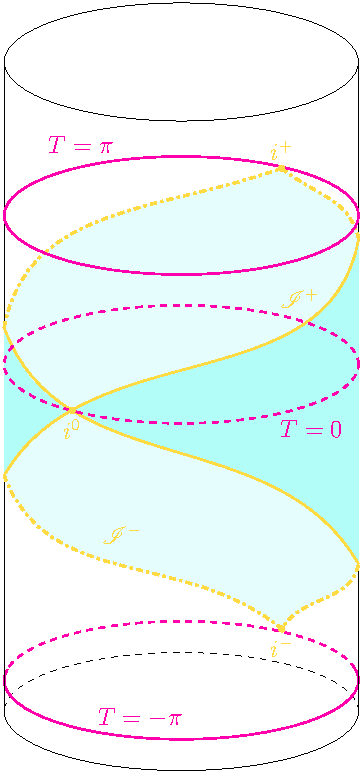
\includegraphics[scale=0.7]{Immagini/Einstein-universe/Einstein-universe.pdf}
	\caption{A spacetime diagram of Einstein static universe, and Minkowski's immersion.}
	\label{fig:Einstein-static-universe}
\end{wrapfigure}

It can be noticed that all timelike geodesics of Minkowski spacetime begin at \(i^-\) and end at \(i^+\), null geodesics go from \(\mathscr{I}^-\) to \(\mathscr{I}^+\), while spacelike geodesics begin and end at \(i^0\).

From this definition of conformal infinity of Minkowski spacetime it's possible formulate precise asymptotic conditions on physical fields representing the exterior field resulting from a localized source, simply requiring that a suitable power of the conformal factor \(\Omega^{-1}\) (the exact power depends on the stringency of the asymptotic condition and on the physical field under consideration), times the field itself can be extended to conformal infinity \(\partial O\) in a suitably well-behaved manner.

With these conditions, quantities which used to be the result of limits such as \(r\rightarrow +\infty\) or \(v\rightarrow \infty\) are now represented as ordinary tensor fields on \(\partial O\). This is a very satisfactory solution to the second problem that was pointed out in the introduction of this section, namely in which direction the limit to spatial infinity should be taken.

We then turn to the first problem, defining the notion of \emph{asymptotically flat} curved spacetime.

The key idea is exactly that the ability to perform an immersion of Minkowski spacetime into Einstein static universe via a conformal isometry crucially depends on the property ``at infinity'' of the spacetime. The idea is then to \emph{define} a spacetime to be \emph{asymptotically flat} if we can perform any similar construction, namely if there is a conformal isometry that maps the original spacetime into an ``unphysical'' manifold \((\tilde{M}, \tilde{g}_{\mu\nu})\) with properties similar to the Minkowski case.
In this way we would clearly solve both problems mentioned at the beginning of the section, since we would have a manifestly invariant formulation of asymptotic flatness, and we have a precise framework to define the concept of ``infinity''.

\begin{remark}
	However, there are some differences that must be pointed out with respect to the Minkowski spacetime. There are mainly \(2\) important remarks:
	\begin{enumerate}[label=(\Roman*)]
		\item We don't want to impose that a spacetime becomes flat at a ``\emph{fixed} position at early or late times'', therefore we cannot expect timelike future \(i^{+}\) or past infinity \(i^{-}\) to be similar to those of Minkowski. Then, we won't ask for any restriction on the structure of curved spacetime related to the presence of these \(2\) points.
		\item  Even if we want to impose the metric to become flat at spatial infinity, smoothness - or even differentiability- are too strong requirements. Then, even if the conformal infinity of asymptotically flat spacetimes is required to contain \(i^0\), the smoothness properties that hold in the Minkowski case must be significantly weakened.
	\end{enumerate}
\end{remark}

All that has been said up to here is enough to give us the fundamental ideas with which we will need to work, but for the sake of completeness we conclude this section with a formal definition of asymptotic flatness. The reader interested in further comments can refer to the already cited chapter \(11\) of~\cite{wald2010general}, or even to the rather technical discussion of Ashtekar \emph{et.al}~\cite{ashtekar1978unified}.
\begin{definition}
	A vacuum spacetime is called \emph{asymptotically flat at null and spatial infinity} if there exists a spacetime \((\tilde{M}, \tilde{g}_{\mu\nu})\), with \(\tilde{g}_{\mu\nu}\) \(C^{\infty}\) everywhere except possibly at a point \(i^0\) where it needs to be \(C^{>0}\), and a conformal isometry \(\psi: M \rightarrow \psi(M)\subset \tilde{M}\) with conformal factor \(\Omega\), so that the following conditions are satisfied:
	\begin{enumerate}[label=(\arabic*)]
		\item The first condition is needed to state that in fact \(i^0\) represents exactly spatial infinity: \(\bar{J^+}(i^0) \cup \bar{J^-}(i^0) = \tilde{M} \setminus M\). Here \(\bar{J^+}(i^0)\) is the closure of \(J^+(i^0)\) and for notational simplicity we write \(M\) instead of \(\psi(M)\). Then \(i^0\) is spacelike related to any point in \(\dot{M}\), and the boundary \(\partial M\) is made of the union  of \(i^0\), \(\mathscr{I}^+ \coloneqq \partial J^+(i^0) \setminus i^0\) and \(\mathscr{I}^- \coloneqq \partial J^-(i^0) \setminus i^0\).
		\item We need to require that no causal pathologies occur near infinity; namely there exists an open neighborhood \(V\) of \(\partial M = i^0 \cup \mathscr{I}^+ \cup \mathscr{I}^-\) such that the spacetime \((V, \tilde{g}_{\mu\nu})\) is strongly causal.
		\item We want \(\Omega\) to be well defined near infinity, so we ask it to be able to be extended to a function on all \(\tilde{M}\) so that it is \(C^2\) at \(i^0\) and \(C^{\infty}\) anywhere else.
		\item \begin{enumerate}
			\item \(\Omega = 0\) at \(\mathscr{I}^+\) and \(\mathscr{I}^-\), with \(\tilde{\nabla}_{\mu} \Omega = 0\).
			\item \(\Omega = 0\) at \(i^0\), with \(\lim_{i^0} \tilde{\nabla}_{\mu} \Omega = 0\) and \(\lim_{i^0} \tilde{\nabla}_{\mu} \tilde{\nabla}_{\nu}\Omega = 2\tilde{g}_{\mu\nu}(i^0)\).
			\end{enumerate}
			The requirement of \(\Omega\) vanishing on \(\partial M\) is saying that at those points an ``infinite stretching'' is involved in going from the unphysical \(\tilde{g}_{\mu\nu}\) to the physical \(g_{\mu\nu}\), so \(i^0\), \(\mathscr{I}^-\) and \(\mathscr{I}^+\) truly represent the infinity of the physical spacetime. Furthermore the requirements on the derivatives of \(\Omega\) imply that the physical metric becomes flat at as one goes to infinity.
		\item Finally, the last requirement is really a technical hypothesis, which is sort of stating that \(\mathscr{I}^+\) and \(\mathscr{I}^-\) have the ``right size''.
		\begin{enumerate}
			\item The map of null directions at \(i^0\) into the space of integral curves of \(n^{\mu} = \tilde{g}^{\mu\nu} \tilde{\nabla}_{\nu}\Omega\) on  \(\mathscr{I}^+\) and \(\mathscr{I}^-\) is a diffeomorphism. This is needed to say that \(\mathscr{I}^+\) and \(\mathscr{I}^-\) have topology \(S^2\times\R\).
			\item For any smooth function \(\omega\) on \(\tilde{M} \setminus i^0\), with \(\omega > 0\) on \(M \cup \mathscr{I}^+ \cup \mathscr{I}^- \) and such that \(\tilde{\nabla}_{\mu}(\omega^4n^{\mu}) = 0\) on \(\mathscr{I}^+ \cup \mathscr{I}^-\), the associated vector field \(\omega^{-1}n^{\mu}\) is complete over \(\mathscr{I}^+ \cup \mathscr{I}^-\). This condition is saying that ``all \(\mathscr{I}^+\) and \(\mathscr{I}^-\) are present'' in the conformally completed spacetime.
			\end{enumerate}
	\end{enumerate}
\end{definition}

As one last observation concerning this section, we remark that we can separately define asymptotically flat spacetimes only at \emph{spatial} or \emph{null} infinity, by simply eliminating the irrelevant parts on the definition above.
Finally, as pointed out by Wald, the definition of \emph{weak asymptotically simplicity} given by Penrose in~\cite{penrose1965zero}, and often taken as a criterion for asymptotic flatness, is formally different but implies all the conditions of the above definition, apart from \((5b)\); this last one is needed in order to make sure that asymptotic flatness does not cease to hold even at finite retarded time~\cite{geroch1978asymptotically}.

\section{Strong Asymptotic Predictability}
In order to study some properties of black holes we first need a precise definition of these objects. The first idea would be to translate the concept of ``regions of no-escape'' into the requirement \(B \coloneqq \{p \in M\vert J^+(p)\subseteq B \}\).
However, this is not really satisfying, as in this way \emph{any} causal future, of \emph{any} set, in \emph{any} spacetime would be called a black hole. The key point is that we must take greater care in specifying what regions of spacetime is impossible to ``escape towards'' when trapped in a black hole.

The clever idea is that for asymptotically flat spacetimes, the impossibility of escaping to future null infinity \(\mathscr{I}^+\) provides an appropriate definition of black hole. Going into more detail, we are saying that \(J^-(\mathscr{I}^+)\) is ``well behaved'' but doesn't include the all physical spacetime. This intuition leads to the following definition:
\begin{definition}
	Let \((M, g_{\mu\nu})\) be an asymptotically flat spacetime with associated unphysical spacetime \((\tilde{M}, \tilde{g}_{\mu\nu})\). We say that \((M, g_{\mu\nu})\)  is \emph{strongly asymptotically predictable} if in the unphysical spacetime there is an open region \(\tilde{V} \subset \tilde{M}\), with the closure \(\overline{M \cap J^-(\mathscr{I}^+)}\subset \tilde{V}\) such that \((\tilde{V}, \tilde{g}_{\mu\nu})\) is globally hyperbolic.
\end{definition}
\begin{remark}
	Here the closure is taken in \(\tilde{M}\), so in particular \(i^0 \in \tilde{V}\). 
\end{remark}
\noindent
Finally we are able to define what a black hole is from a topological point of view.
\begin{definition}
	A strongly asymptotically predictable spacetime \((M, g_{\mu\nu})\) is said to contain a \emph{black hole} if \(M\) is not contained in \(J^-(\mathscr{I}^+)\). Consequently the \emph{black hole region} is defined as 
	\[
	B \coloneqq M \setminus J^-(\mathscr{I}^+)
	\]
	and the boundary of \(B\) is called the \emph{event horizon} \(H\coloneqq \partial J^-(\mathscr{I}^+) \cap M \).
\end{definition}

\begin{remark}
	Let us make a couple of remarks concerning why it is important to make some assumptions to give the definition of such objects.
	\begin{enumerate}[label=(\Roman*)]
		\item The notion of asymptotic flatness is needed to specify a definition of the ``infinity'' that observers trapped in a black hole no longer have any hope of reaching. The definition might be extended in some cases where a suitable notion of ``infinity'' is provided, but we are not able to say anything in general.
		\item The requirement for strong asymptotic predictability is more an instrumental physical hypothesis, rather than a mathematical one, needed for well-posedness. It is really meant to ensure that physics is predictable on and outside \(H\).
		
		Indeed, asymptotically flat spacetimes which fail to be strongly predictable are said to contain a \emph{naked singularity}, but these cases are believed not to be physically relevant. This statement is the main content of the Cosmic Censorship Conjecture: the curious reader may find its definition in chapter \(12\) of~\cite{wald2010general} and endless literature browsing the internet, starting from~\cite{dias2018strong}.
	\end{enumerate}
\end{remark}

%todo: si potrebbe fare una pagina di disegnini, tipo pag. 300 del wald

\section{Black Holes evaporation}
\label{sec:black-holes-evaporation}
Gravity - or equivalently, curvature - can have dramatic consequences on observers living at different locations, and in particular can change to a remarkable extent; even the basic notions a na\"ive physicist would take for granted; if Einstein revolutionized the world by showing how simultaneity is a luxury reserved to ``slow'' observers, even a common notion of time has to be completely ripped up for those who live in non-stationary spacetimes... such as ours.

\noindent
The absence of a common timelike killing vector field, arising from an eventual time translation-symmetry, leaves two distant observers - as the ones separated by some process of gravitational collapse - unable to agree on a common notion of time, with important consequences on the description of the physical phenomena they can see.
Nevertheless, there is a situation where much of the treatment we are used to in Minkowski spacetime can be retrieved: if the spacetime possesses asymptotically flat regions in the past and the future, one can naturally define and \emph{in} and \emph{out} region where a local notion of time can be defined, and all the quantum field theory machinery we are used to can work pretty much the same way.
However, the two different notions of ``time'' in the \emph{in} and \emph{out} region will remain distinguishable.

The most dramatic effect of this discrepancy is that two observers living in these separated regions will not agree on the notion of \emph{vacuum}: a state which contains no particles for observer \(A\) in \emph{in}, might not look empty to observer \(B\) in \emph{out}.
Then of course, the all Fock space and the ladder operators will be different for \(A\) and \(B\), even if they can still be connected by a Bogoliubov transformation.

The most astonishing consequence of this discrepancy is the so-called \emph{Hawking radiation}. With an incredibly modern approach, in \(1974\) Hawking predicted that indeed, an observer in the future region of a spacetime where gravitational collapse gives rise to a black hole, shall observe a thermal radiation with a Planck spectrum of Hawking temperature \(T_H\). Both the thermal spectrum of the radiation and the precise computation of the temperature arise from the analysis of the coefficient of the above mentioned Bogoliubov transformation. For additional details on this process, we shall refer to the original article~\cite[]{hawking1975particle} or chapter \(3\) of the book by Fabbri and Navarro~\cite[]{fabbri2005modeling}, where they introduce the topic in a very pleasantly didactic way.

The temperature of the Planck spectrum of the radiation can also be retrieved through a very neat and famous argument due to Gibbons and Hawking~\cite[]{gibbons1993action}; when carrying out a Wick rotation in a black hole solution, in order to avoid the insurgence of a conical singularity, one must impose a periodicity of the Euclidean time coordinate corresponding to exactly the Hawking temperature:

\begin{equation}
	\label{eq:hawking-temperature}
	T_H = \frac{\hbar c^3}{8\pi Gk_B}\frac{1}{M}.
\end{equation}

\begin{remark}
	It stands out immediately that the temperature in~\eqref{eq:hawking-temperature} is proportional to \(\hbar\). In particular then, in the semiclassical limit, as \(\hbar \rightarrow 0\) also \(T_H \rightarrow 0\), and no Hawking radiation is left. This is precisely what we refer to when we say that Hawking radiation is a purely quantum mechanical effect.
\end{remark}

According to the classical study of any radiation with Planck spectrum, each angular momentum component of the fields gives a contribution to the luminosity
\[
L_{\ell} = \frac{2\ell + 1}{2\pi} \int_0^{+\infty} d\omega \frac{\hbar\omega}{e^{8\pi M\omega} - 1}	d\omega  = (2\ell + 1) \cdot\frac{\hbar}{768\pi M^2}.
\]
However, simply summing up all the contributions would lead to a divergent result; as motivated in~\cite[]{fabbri2005modeling} - among others - this is because we are neglecting backscattering. This is basically equivalent to saying that we are neglecting backreaction, and so we would have a black hole radiating forever: if not in the luminosity here we would get a divergence in the total emitted energy, in clear contrast with the finite amount contained within the black hole.

Backscattering effects are resumed by the \emph{gray-body factors} \(\Gamma_{\omega, \ell}\), that weight the energy distribution and decrease with \(\ell\). They could be estimated via the Page approximation~\cite[]{page1976particle}:
\[
	\Gamma_{\omega,\ell} \approx 16(\omega M)^{2\ell + 2}\left(\frac{\ell!^3}{(2\ell)!(2\ell + 1)!}\right)^2,
\]
from which it is evident that the most relevant contribution is given by the \(s-\)wave mode:
\[
\Gamma_{\omega, 0} \approx 16\omega^2M^2 \implies L_{\ell = 0} = \frac{\hbar}{7680\pi M^2}.
\]
This represent about \(90\%\) of the contribution to Hawking radiation, as it turns out by more careful computations of luminosity, which involve contributions from higher angular momenta, from higher spin species, or refinement of the Page approximation via numerical methods.
Once the luminosity has been computed, via energy conservation it is possible to immediately infer what is the decreasing rate of the mass of the black hole; reintroducing the units:
\begin{equation}
	\label{eq:evaporation-rate}
	R_{ev} = -\frac{1}{M}\frac{dM}{dt} = (8\pi)^3\beta \frac{G}{\hbar^2c^5}\left(k_BT_H\right)^3
\end{equation}

where \(\beta \sim \mathcal{O}(10^{-5})\) hides the precise knowledge of backscattering. Apart from irrelevant coefficients of order \(1\), this shall also coincide with the expected rate of contraction of the area of the horizon, \(\frac{\delta\mathcal{A}}{\mathcal{A}}\).


\subsection{Causality violation}
\label{subsec:causaliy-bh-evaporation}
It has been pointed out (first of all by Kodama~\cite{Kodama:1979vm}) that Black Hole evaporation is in tension with global hyperbolicity: in fact the region formed after the complete evaporation of the black hole would cause a ``chronology violation'', in the sense that the initial data collected on a Cauchy surface might not be enough to predict the evolution after the disappearance of the singularity.

\begin{wrapfigure}{r}{0.45\textwidth}
	\centering
	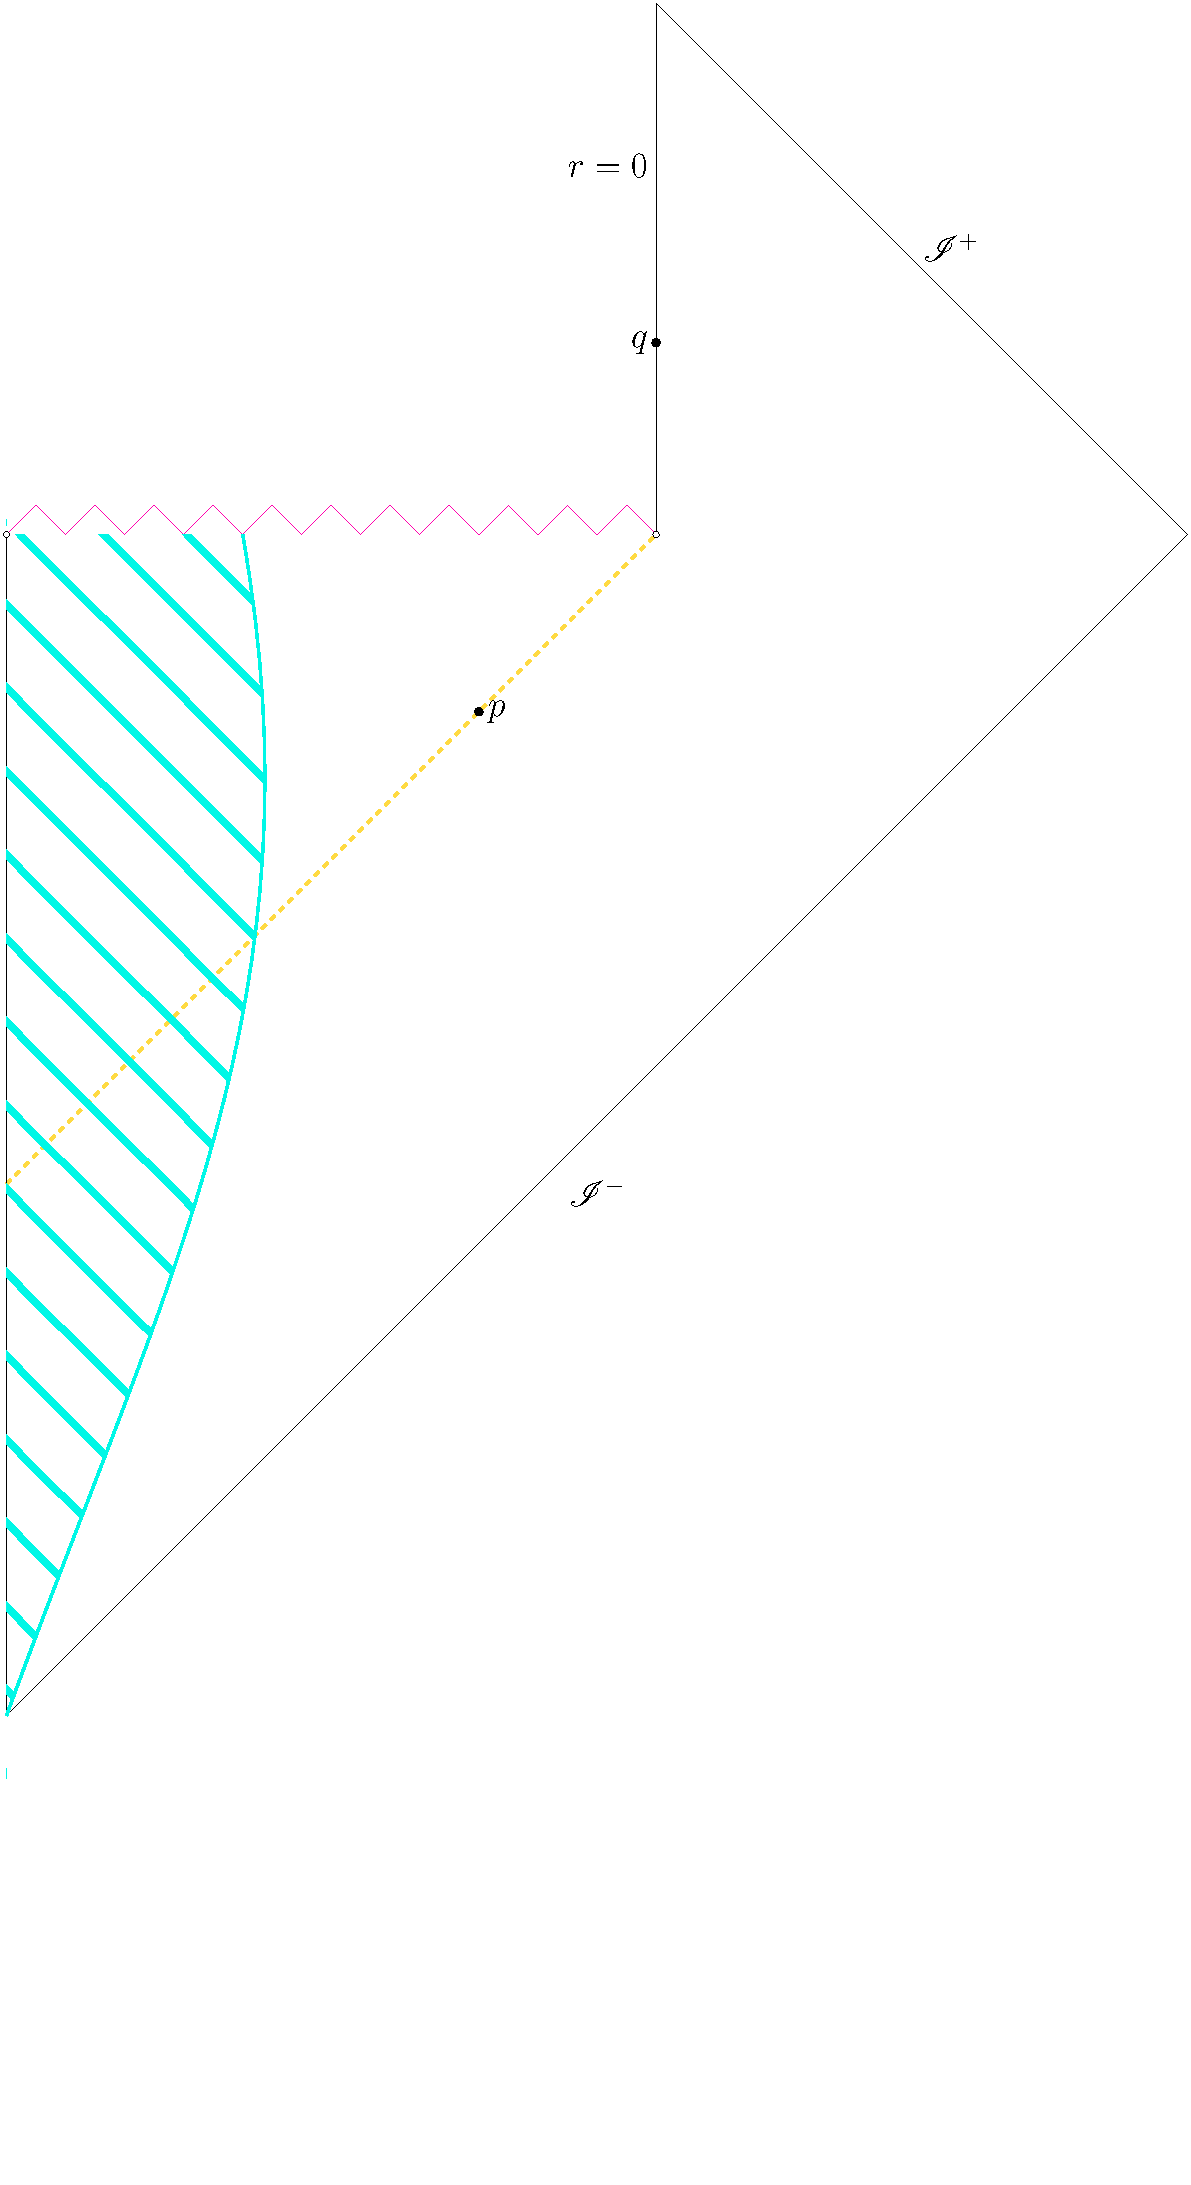
\includegraphics[scale=0.3]{Immagini/evaporating-black-holes/evaporating-black-holes.pdf}
	\caption{chronology violation after black hole evaporation: the is information coming out from the singularity as well! The presence of that extra triangular in the Penrose diagram shows that there exist pair of points for which future reflectivity doesn't hold anymore.}
\end{wrapfigure}

Such an hypothesis was assumed also for the original Black Hole Area theorem: in that context it wasn't incoherent, as the classical black hole area theorem is forbidding evaporation; however, we will see that this won't be the case for us, and therefore it is necessary to briefly discuss the consistency of our hypotheses.

The problem might be easily worked around by observing that we only need to require global hyperbolicity for the region the horizon lies into. This wouldn't bring about any contradiction, as the chronology violation region only begins \emph{after} the complete evaporation of the black hole, where no horizon exists anymore. For the readers concerned about the scarce punctiliousness of the above statement, we have good news: it is possible to do even better than that! 

As already commented by Hawking and Ellis in~\cite[]{hawking1973large} (for Penrose's theorem, but it will be the same for our generalized area theorem), the global hyperbolicity assumption is only used to ensure that \((M, g)\) is causally simple, so that the generators a surface \(K\), \(\partial J^+(\mathscr{K})\) have past endpoints on \(K\) [i.e. \(\partial J^+(K) = H^+(K)\)].
In~\cite{minguzzi2020gravitational} Minguzzi provides a coherent framework within which singularity formation can be derived. He argues that the hypothesis of global hyperbolicity can be relaxed to \emph{past reflectivity} and \emph{openess}, because what really is needed is a topological condition that prevents the horizon from ``swallowing up'' the all universe. We believe that the same framework can be adapted to our work as well, but in order to show it, we need to dig a little bit deeper into the causal properties of spacetimes.

\subsection{Past reflectivity}
	\label{subsec:past-reflectivity}
	Let us start with the definition of future reflectivity.
	\begin{definition}
		The spacetime \((M,g)\) is \emph{future reflecting} if any of the following equivalent properties holds true. For each \(p, q\in M\):
		\begin{enumerate}
			\item \(p\in \overline{ J^-(q)} \implies q\in \overline{J^+(p)}\);
			\item  \(p\in \partial J^-(q) \implies q\in \partial J^+(p)\);
			\item \(I^-(p) \subset I^-(q) \implies I^+(q) \subset I^+(p)\);
			\item \(\uparrow I^-(p) = I^+(p)\);
			\item the volume function \(\iota^+(p) = - \mu(I^+(p))\) is continuous.
		\end{enumerate}
	\end{definition}
	Here \(\uparrow I^-(p) \coloneqq Int\left[\cap_{r\in I^-(p)}I^+(p)\right]\) is the \emph{common future}, while \(\mu\) is any finite spacetime measure absolutely continuous with respect to the Lebesgue measure induced by the coordinate charts. Past reflectivity is defined similarly.

	Future and past reflectivity are implied by \emph{causal continuity}, and hence by global hyperbolicity as well. We shall now show that an evaporating black hole spacetime is still \emph{past reflecting}, but not \emph{future reflecting}. Lesourd had already shown in~\cite[]{lesourd2018causal} that future reflectivity cannot be
	maintained in the presence of any evaporating null hypersurface, not just the specific case of the black hole horizon. 

	But what is an evaporating null hypersurface then? Minguzzi observes that typically, what distinguishes an evaporating black hole is that the observer who escapes the fate of falling into it has the possibility to see the process of gravitational collapse coming to an end. This is in stark contrast with what happens in Schwarzschild, where an asymptotically far observer would see any object falling towards the horizon for an infinite time, without ever reaching it.

	\begin{figure}
		\centering
		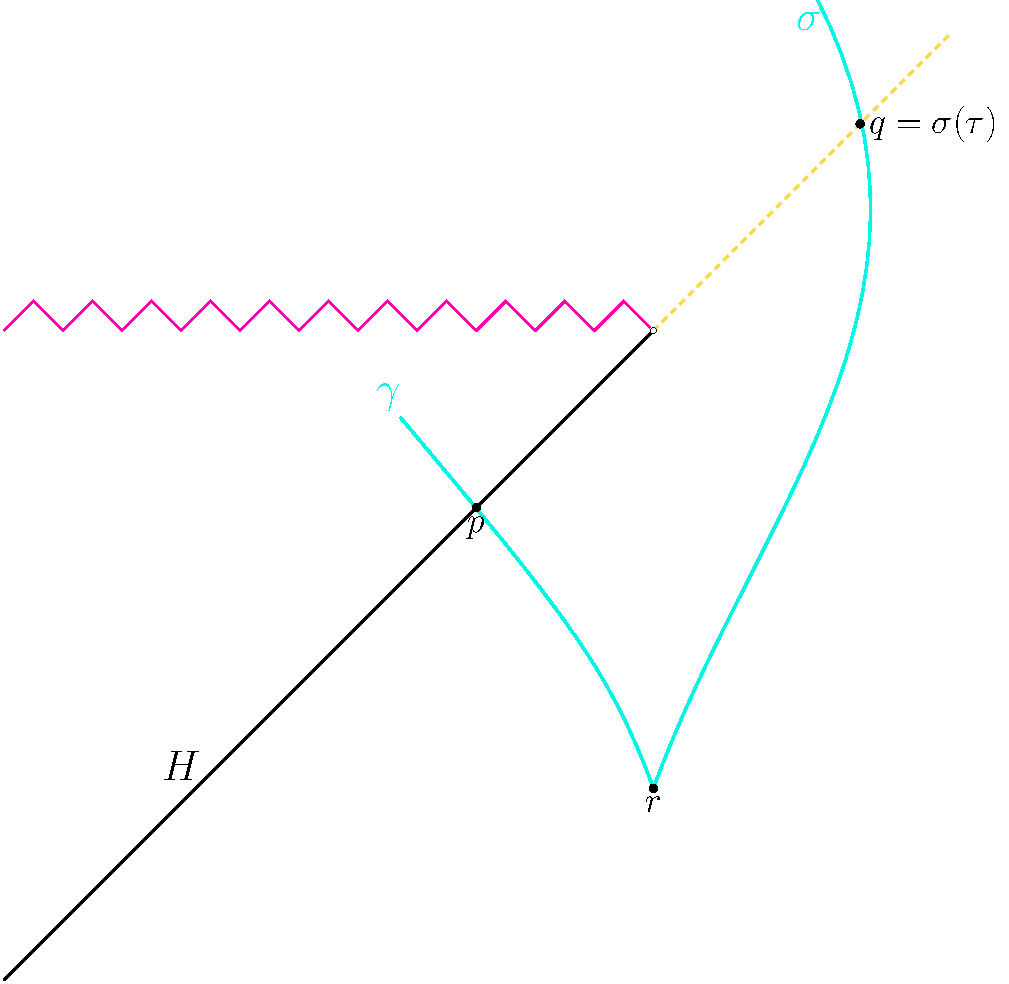
\includegraphics[scale=0.5]{Immagini/evaporating-surfaces/evaporating-surfaces.pdf}
		\caption{structure of evaporating null hypersurfaces.}
		\label{fig:evaporating-surface}
	\end{figure}

	Let us refer to~\ref{fig:evaporating-surface} to formalize that idea: two timelike curves leaves \(r\), \(\gamma\) falling into the black hole, while \(\sigma\) is future inextendible. Minguzzi is interested in those observers who can witness the whole falling history, \(\gamma ([0,a)) \subset J^-(\sigma([0,t]))\).

	\begin{definition}
		The horizon \(H\) at point \(p\) is evaporating from the point of view of observer \(\sigma\) if there exists \(t > 0\) such that
		\[
		\gamma \left([0, a]\right) \subset J^-\left(\sigma\left([0, t]\right)\right).	
		\] 
	\end{definition}
	Now the following becomes more intuitive
	\begin{theorem}
		Past reflecting spacetimes which contain an evaporating \(C^0\) future null hypersurface \(H\) are not future reflecting.
	\end{theorem}
	Define \(\tau \coloneqq \inf t\) for which the inclusion \(gamma \left([0, a]\right) \subset J^-\left(\sigma\left([0, t]\right)\right)\), holds, and \(q = \sigma(\tau)\), as in figure~\ref{fig:evaporating-surface}.
	Past reflectivity is necessary to ensure that points to the future of \(q\) can see \(\gamma[0,a)\), and hence, \(p\) to their past, but future reflectivity fails because if any point to the future of \(q\) was in the future of \(p\), it would create a contradiction with the definition of horizon \(H\). 
	\begin{remark}
		It is interesting to notice that past reflectivity is not a causality condition (it does not belong to the ladder of causality definitions), but instead should be regarded as a restriction on \emph{how} information can propagate in the universe.
	\end{remark}

	Now he defines a couple of convenient definitions.
	\begin{definition}
		A \emph{future lightlike S-ray} is a future inextendible causal curve which starts from \(S\) and does not intersect \(I^+(S)\). A non-empty set \(S\) is a \emph{future null araying set} if there are no future lightlike S-rays. 
	\end{definition}
	It can be shown that compact null araying set lying in the non-vicious region implies that the surface is trapped, and under very weak causality assumptions (like strong causality) the converse becomes true as well. Moreover
	\begin{definition}
		A compact non-empty set S that does not intersect the chronology violation region \(\mathcal{C}\) is said to have an \emph{unavoidable} or \emph{swallowing} horizon if there exists an open neighborhood U of \(H^+(S)\) such that its past in \(U\) is strictly contained in the past domain of dependence of \(H^+(S)\) 
		\[
			I^-_U(H^+(S)) \subset Int D^-(H^+(S)).	
		\]
	\end{definition}
	Under this condition any observer that were to pass through a neighborhood of the horizon \(H^+(S)\) would be forced to intersect it, and hence fall under its causal influence. This is a topological feature that we wish to avoid for the horizons that we study. In particular it can be proved that null future araying sets in the non-vicious region have unavoidable horizons.

	What is more similar to an actual causality condition, and that seems to be the other minimal requirement, is
	\begin{definition}
		A spacetime is \emph{(spatially) open} if it does not contain a compact spacelike hypersurface.
	\end{definition}	
	In particular spacetimes with non-compact Cauchy hypersurfaces are \emph{open}, so global hyperbolicity also implies this new feature. 
	Finally, theorem \(2.10\) of~\cite[]{minguzzi2020gravitational} states:
	\begin{theorem}
		Let \((M,g)\) be a past reflecting and open spacetime. Then it does not admit compact future null araying sets that do not intersect \(\mathcal{C}\).
	\end{theorem}
	This is really the result that we need: in fact this will guarantee us the existence of prompt curves that reach the conformal null infinity, lying on the boundary of the future of compact surfaces \(\partial J^+(K)\) in the non-vicious region, that cannot be null araying.